\ofsubsection{Blitzball}
%
\ofquote{"Os jogadores lutam com toda sua força: os fãs torçem pelo seu time favorito. Eles equecem da dor, do sofrimento... somente o jogo importa! Esse é o porquê Blitz está vivo por tanto tempo. Pelo menos é o que acho."\\}{Wakka}\\\\
%
\accf{Blitzball} é um esporte de grupo que pode ser comparado ao polo aquático, exceto que se é jogado sob a água, dentro de uma grande esfera. 
A água em si é imbuída com propriedades mágicas que permitem aos jogadores ficar submergidos por períodos longos.
Nesse jogo dois times opostos jogam um contra o outro e aquele que pontuar mais, vence.
Um time consiste em um goleiro e de 2 a 5 jogadores.
O jogo parece um combate, exceto que se é focado em controlar a bola.
A ordem de turno é determinado da mesma maneira que no combate, o jogador que age primeiro pega a bola após o pontapé inicial.
Cada partida consiste em dois tempos, em que cada um tem 10 rodadas.
Após terminar o primeiro tempo, os times têm um intervalo em que cada jogador recupera seus pontos de fôlego.
Blitzball é jogado dentro de uma esfera de 15u de diâmetro cheia de água, mas você pode usar um esquema simplificado como mostrado abaixo para ilustrar o jogo.
%
\vfill
%
\begin{figure}[h]
	\centering
	\resizebox{\columnwidth}{8cm}{%
	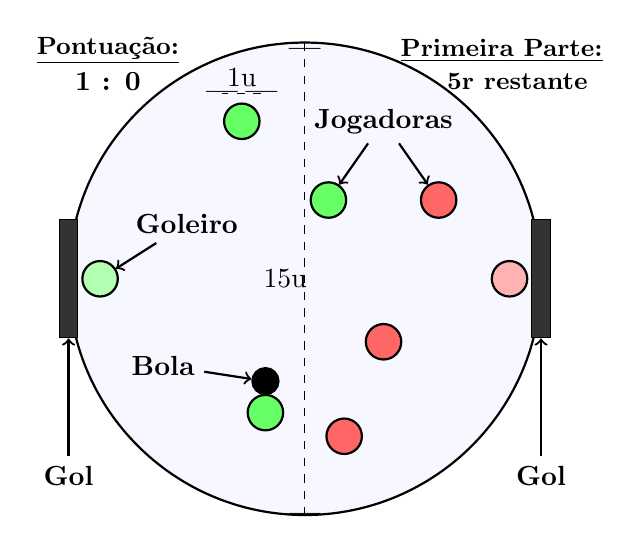
\begin{tikzpicture}[]
	\tikzstyle{test}=[thick, draw, circle, align=center]					
	\node[fill=blue!3!white, test, thick ,minimum size = 6cm](tarea)at (0,0) {};

	\node[fill=red!60!white, test,minimum size = 0.45cm](player2)at (1.7,1) {};
	\node[fill=red!60!white, test,minimum size = 0.45cm](target)at (1,-0.8) {};
	\node[fill=red!60!white, test,minimum size = 0.45cm](target)at (0.5,-2) {};

	\node[fill=green!60!white, test,minimum size = 0.45cm](target)at (-0.8,2) {};
	\node[](a1)at (-0.55,2.35) {\bf |};
	\node[](a2)at (-1.05,2.35) {\bf |};
	\node[](a2)at (-0.8,2.55) {1u};
	\draw[-, dashed](-0.55,2.35) -- (-1.05,2.35);
	
	\node[fill=green!60!white, test,minimum size = 0.45cm](player)at (0.3,1) {};
	\node[fill=green!60!white, test,minimum size = 0.45cm](target)at (-0.5,-1.7) {};
	\node[fill=black, test,minimum size = 0.1cm](ball)at (-0.5,-1.3) {};		
	\node[](tball)at (-1.8,-1.1) {\bf Bola};
	\node[](tplayer)at (1,2) {\bf Jogadoras};
	\draw[->, thick](tball) -- (ball);
	\draw[->, thick](tplayer) -- (player);
	\draw[->, thick](tplayer) -- (player2);
	
	\node[](tgk)at (-1.5,0.7) {\bf Goleiro};
	\node[](tgoal)at (-3,-2.5) {\bf Gol};
	\node[fill=black!80!white, draw, rectangle,minimum height=1.5cm, minimum width=0.05cm](goal)at (-3,0) {};
	\node[fill=green!30!white, test,minimum size = 0.45cm](gk)at (-2.6,0) {};
	\draw[->, thick](tgk) -- (gk);
	\draw[->, thick](tgoal) -- (goal);
	
	\node[](tgoal2)at (3,-2.5) {\bf Gol};
	\node[fill=black!80!white, draw, rectangle,minimum height=1.5cm](goal2)at (3,0) {};
	\node[fill=red!30!white, test,minimum size = 0.45cm](target)at (2.6,0) {};
	\draw[->, thick](tgoal2) -- (goal2);
	
	\node[](se2)at (0,2.9) {\bf ---};
	\node[](se2)at (0,-3) {\bf ---};
	\draw[-, dashed](0,3) -- node[] {}(0,-3);
	\node[](sca)at (-0.25,0) {15u};		
	
	\node[](sca)at (2.5,2.9) {\small\bf\underline{Primeira Parte:}};
	\node[](sca)at (2.5,2.5) {\small\bf\hspace*{0.4cm}5r restante};
	\node[](sca)at (-2.5,2.9) {\small\bf\underline{Pontuação:}};
	\node[](sca)at (-2.5,2.5) {\bf 1 : 0};
	\end{tikzpicture}
	}
\end{figure}
%
\vfill
%
As proficiências do jogador em diferentes aspectos do jogo são definidas pelos 4 atributos a seguir:\ofrow
\accf{Pontos de fôlego (PF):} Representa sua durabilidade durante o jogo.
	A maioria das ações custam uma quantidade de PF para se executar.
	Quando seus PF alcançam 0, você pode continuar jogando, mas não pode realizar ações que custam PF.
%
\ofrow
%
\accf{Ataque (ATQ):} Melhora suas chances de passar e chutar a bola.\ofrow
\accf{Defesa (DEF):} Melhora suas chances de roubar e interceptar a bola.\ofrow
\accf{Velocidade (VE):} Determina o quão rápido você pode nadar.
%
\newpage
%
%\ofquote{"When you got the ball, you gotta score!"\\}{Tidus}
%
%\ofpar
%\begin{center}  \includegraphics[width=\columnwidth]{./art/blitz/stadium.jpg} \end{center}
\includegraphics[width=\columnwidth]{./art/blitz/stadium.jpg}
%
\vfill
%
Durante cada turno, um jogador pode mergulhar uma distância total até sua VE+1 em unidades e realizar uma das seguintes ações.
A única exceção é o goleiro, que fica em frente ao gol o tempo todo e somente reage aos chutes dos inimigos.
O conjunto de ações que você pode realizar muda a depender de se você tem ou não a bola.
%
\ofrow
%
\accf{Passe:} Você passa a bola a outro jogador.
A bola pode viajar uma distância máxima igual a seu ATQ+1d em unidades.
Enquanto realizando o passe, cada oponente dentro de 1u de você pode tentar bloquear a bola.
Ao fazer isso, cada bloqueador reduz a distância do passe pela sua DEF+1d.
Se essa distância for reduzida a 0, ele pega a bola.
Se a bola passa de todos os bloqueadores, mas não alcança seu alvo, o jogador mais próximo a pega.
%	
\ofrow
%
\accf{Chute:} Você chuta a bola ao gol.
A bola pode viajar uma distância máxima igual a seu ATQ+1d em unidades.
Primeiro, cada chute pode ser bloqueado por oponentes próximos da mesma maneira que o passe. Assim, se a bola alcança o gol, o goleiro pode tentar pegá-la.
Se a DEF+1d do goleiro é maior do que a distância restante da bola, ele a pega, do contrário você pontua.
Se o goleiro pega a bola, ele pode imediatamente fazer um passe que não pode ser bloqueado. Se um ponto foi marcado, então um novo pontapé inicial será realizado ao inicio da próxima partida.
Cada chute custa a você uma quantidade de PF igual ao seu ATQ.
%	
\ofrow
%
\accf{Encontrão:} Você rouba a bola de um jogador que esteja a 1u.
Se sua DEF+1 é maior do que a DEF+1d do alvo, então você rouba a bola com sucesso. Também, adicione 1d à sua rolagem, para cada encontrão que o alvo receber desde seu último turno.
Ao realizar o encontrão, você também pode disparar a uma distância de sua VE+1 em unidades.
Cada encontrão custa uma quantidade de PF igual à sua DEF.
%
\ofrow
%	
\accf{Técnica:}
Técnicas são habilidades especiais que podem te ajudar a vencer um jogo.
Cada técnica contém seu efeito e custo em PF na sua descrição.
Uma lista de técnicas é mostrada na próxima página.
%
\vfill
%
Durante o jogo, os jogadores podem sofrer os seguintes efeitos por uma duração limitada.\ofrow
\accf{Veneno:} No início de cada turno, seu PF atual é reduzida em 10\% de seu máximo.\ofrow
\accf{Enfraquecido:} Seu ATQ, DEF e PF são reduzidos pela metade.\ofrow
\accf{Soneca:} Seus turnos são pulados e você não pode pegar ou bloquear a bola.
Quando um jogador passa para você enquanto estiver dormindo, você acorda e a bola é recebida pelo jogador mais próximo.
%
\clearpage
%
\ofquote{"Este é o chute Jecht, não é?"\\}{Yuna}\ofpar
%
\includegraphics[width=\columnwidth]{./art/blitz/ingame.jpg}
%
\ofpar
%
Todos os atributos de um jogador de Blitzball são derivados e melhorados pelos seus atributos de combate como a seguir:\ofrow
\accf{Pontos de fôlego = Pontos de vida + Pontos de mana} \ofrow
\accf{Ataque = Força + Magia} \ofrow
\accf{Defesa = Defesa (físca) + Resistência} \ofrow
\accf{Velocidade = Agilidade} \ofrow
%
Então se um personagem jogador aumenta de nível fora de uma partida e ganha FOR+1, seu ATQ também é aumentado em +1.
Para evitar confusão, os atributos de Blitzball devem ser acompanhados separadamente daqueles de combate.
No início cada jogador já sabe uma técnica a sua escolha.
Cada jogador aprende até 3 técnicas no máximo, ao observar outros jogadores que as executam.
Se durante uma partida, alguém a 3u de você executa uma técnica, você pode tentar passar num teste de DF~9 para aprendê-la.
Se já conhecer 3, você pode esquecer uma delas para substituir pela nova. Jogar Blitzball é uma fonte de experiência para os personagens jogadores, o que os ajudam a alcançar marcos na aventura mais rapidamente.
Além do mais, vencedores do Blitzball são normalmente premiados com várias recompensas e prêmios, incluindo equipamentos, itens e Gil.
%
\vfill
%
\oftable{p{0.15\columnwidth} l p{0.73\columnwidth}}
{\accf{Técnica} & \accf{PF} & \accf{Efeito}}
{
	Chute Jecht & 20 & Você dá um chute que não pode ser bloqueado, exceto pelo goleiro.\ofrow
	Luvas de agarrar & 8 & Até o inicio de seu próximo turno, adicione 1d a sua DEF enquanto tenta pegar um passe ou chute. \ofrow
	Parrudo & 8 & Até o fim de seu próximo turno, sua DEF aumenta em um valor igual a seu ATQ.\ofrow
	Espírito dos\newline auroques & 12 & Todos os aliados dentro de 5u aumentam seu ATQ e DEF em 3 até o início de seu próximo turno. \ofrow
	Passe\newline drenante & 8 & Você passa a bola, em que se adiciona 3u à distância dela. Cada jogador que falhar ao interceptar a bola, perde 5 PF e seu PF aumenta na mesma quantidade.\ofrow
}
%
\newpage
%
\oftable{p{0.16\columnwidth} l p{0.73\columnwidth}}
{\accf{Técnica} & \accf{PF} & \accf{Efeito}}
{
%	Jecht Shot & 20 & You make a shot, that cannot be blocked by any player except the goalkeeper.\ofrow
	Chute\newline esfera & 15 & Chute e adiciona 2d em unidades a distância da bola.\ofrow
	Chute\newline voleio & 6 & Ao receber um passe ou pegar a bola antes do início de seu próximo turno, você pode chutar imediatamente. \ofrow
	Chute\newline venenoso & 10 & Chute e adiciona 3u à distância da bola. Cada jogador que tentar bloqueá-la faz um teste de DF~8 ou fica envenenado por 3 rodadas.\ofrow
	Chute Enfraquecedor & 10 & Chute e adiciona 3u à distância da bola. Cada jogador que tentar bloqueá-la faz um teste de DF~8 ou fica Enfraquecido por 3 rodadas.\ofrow
	Chute\newline soneca & 10 & Chute e adiciona 3u à distância da bola. Cada jogador que tentar bloqueá-la faz um teste de DF~8 ou fica Dormindo por 3 rodadas.\ofrow
	Passe Enfraquecedor & 8 & Passe e adiciona 3u à distância da bola. Cada jogador que tentar bloqueá-la faz um teste de DF~8 ou fica Enfraquecido por 3 rodadas. \ofrow
	Passe\newline venenoso & 8 & Passe e adiciona 3u à distância da bola. Cada jogador que tentar bloqueá-la faz um teste de DF~8 ou fica Envenenado por 3 rodadas. \ofrow
	Passe\newline soneca & 8 & Passe e adiciona 3u à distância da bola. Cada jogador que tentar bloqueá-la faz um teste de DF~8 ou fica Dormindo por 3 rodadas.\ofrow
	Encontrão\newline venenoso & 10 & Dê um encontrão e adiciona +3 à sua DEF atual. Cada jogador que tentar bloqueá-la faz um teste de DF~8 ou fica Envenenado por 3 rodadas.\ofrow
	Encontrão\newline soneca & 10 & Dê um encontrão e adiciona +3 à sua DEF atual. Cada jogador que tentar bloqueá-la faze um teste de DF~8 ou fica Dormindo por 3 rodadas.\ofrow
	Encontrão Enfraquecedor & 10 & Dê um encontrão e adiciona +3 à sua DEF atual. Cada jogador que tentar bloqueá-la faz um teste de DF~8 ou fica Enfraquecido por 3 rodadas. \ofrow
	Encontrão\newline drenante & 10 & Dê um encontrão e adiciona +3 à sua DEF atual. Cada jogador que tentar bloqueá-la faz um teste de DF~8 ou seu PF é reduzido em -5 e o seu PF aumenta na mesma quantidade.\ofrow
	Encontrão\newline escorrega & 7 & Até o início do seu próximo turno, cada oponente que tentar dar um encontrão em você tem que fazer um teste de DF~8 primeiro ou errará o encontrão.\ofrow
	Defesa \newline de Elite & 8 & Até o início de seu próximo turno, quando um oponente se mover dentro de 1u de você, você pode dar um encontrão nele imediatamente.\ofrow
}
%
\clearpage